\documentclass[useAMS,usenatbib]{mn2e}
\usepackage{amsmath}
\usepackage{amssymb}
\usepackage{graphics}
\usepackage{graphicx}
\usepackage{epsfig} 
\usepackage{hyperref}
\def\be{\begin{equation}}
\def\ee{\end{equation}}
\def\ba{\begin{eqnarray}}
\def\ea{\end{eqnarray}}

% To highlight comments
\usepackage{color}
\definecolor{red}{rgb}{1,0.0,0.0}
\newcommand{\red}{\color{red}}
\definecolor{blue}{rgb}{0.1,0.3,0.9}
\newcommand{\blue}{\color{blue}}

\usepackage[normalem]{ulem}
\definecolor{darkgreen}{rgb}{0.0,0.5,0.0}

\newcommand{\documentname}{paper~}
\newcommand{\LCDM}{$\Lambda$CDM~}
\newcommand{\beq}{\begin{eqnarray}} 
\newcommand{\eeq}{\end{eqnarray}} 
\newcommand{\zz}{$z\sim 3$}

\newcommand{\apj}{ApJ} 
\newcommand{\apjs}{ApJS} 
\newcommand{\apjl}{ApJL} 
\newcommand{\aj}{AJ} 
\newcommand{\mnras}{MNRAS} 
\newcommand{\mnrassub}{MNRAS accepted} 
\newcommand{\aap}{A\&A} 
\newcommand{\aaps}{A\&AS} 
\newcommand{\araa}{ARA\&A} 
\newcommand{\nat}{Nature} 
\newcommand{\physrep}{PhR}
\newcommand{\pasp}{PASP}   
\newcommand{\pasj}{PASJ}   
\newcommand{\avg}[1]{\langle{#1}\rangle} 
\newcommand{\ly}{{\ifmmode{{\rm Ly}\alpha}\else{Ly$\alpha$}\fi}}
\newcommand{\hMpc}{{\ifmmode{h^{-1}{\rm Mpc}}\else{$h^{-1}$Mpc }\fi}} 
\newcommand{\hGpc}{{\ifmmode{h^{-1}{\rm Gpc}}\else{$h^{-1}$Gpc }\fi}} 
\newcommand{\hmpc}{{\ifmmode{h^{-1}{\rm Mpc}}\else{$h^{-1}$Mpc }\fi}} 
\newcommand{\hkpc}{{\ifmmode{h^{-1}{\rm kpc}}\else{$h^{-1}$kpc }\fi}}
\newcommand{\hMsun}{{\ifmmode{h^{-1}{\rm
        {M_{\odot}}}}\else{$h^{-1}{\rm{M_{\odot}}}$~}\fi}}  
\newcommand{\hmsun}{{\ifmmode{h^{-1}{\rm
        {M_{\odot}}}}\else{$h^{-1}{\rm{M_{\odot}}}$}\fi}}  
\newcommand{\Msun}{{\ifmmode{{\rm {M_{\odot}}}}\else{${\rm{M_{\odot}}}$}\fi}} 
\newcommand{\msun}{{\ifmmode{{\rm {M_{\odot}}}}\else{${\rm{M_{\odot}}}$}\fi}} 
\newcommand{\lya}{{Lyman$\alpha$~}}
\newcommand{\clara}{{\texttt{CLARA}}~}
\newcommand{\rand}{{\ifmmode{{\mathcal{R}}}\else{${\mathcal{R}}$ }\fi}} 
\newcommand{\hs}{{\hspace{1mm}}}
\newcommand{\muavg}{\vert\langle\cos\theta\rangle\vert}
% definition to produce a "less than or similar to" symbol
\def\lsim{~\rlap{$<$}{\lower 1.0ex\hbox{$\sim$}}}

% definition to produce a "greater than or similar to" symbol

% definition to produce a "greater than or similar to" symbol
\def\gsim{~\rlap{$>$}{\lower 1.0ex\hbox{$\sim$}}}

\begin{document}

\title[Bayesian halo concentrations]{Dark matter halo
  concentrations with a bayesian approach}
\author[Poveda \& Forero-Romero]{
\parbox[t]{\textwidth}{\raggedright
  Christian Poveda$^{1}$ \&
  Jaime E. Forero-Romero$^{1}$
}
\vspace*{6pt}\\
$^{1}$Departamento de F\'{i}sica, Universidad de los Andes, Cra. 1
No. 18A-10, Edificio Ip, Bogot\'a, Colombia\\
}
\maketitle

\begin{abstract}
asd
\end{abstract}
\begin{keywords}
methods: numerical, galaxies: haloes, cosmology: theory, dark
matter
\end{keywords}


\section{Introduction}
\label{sec:introduction}


\citep{NFW}


\section{Basic properties of the NFW density profile}
\label{sec:basics}

The Navarro-Frenk-White density profile can be written as

\begin{equation}
\rho(r) = \frac{\rho_c\delta_c}{r/r_s(1+r/r_s)^2}, 
\end{equation}
%
where $\rho_c\equiv 3H^2/8\pi G$ is the Universe critical density,
$\delta_c$ is the halo dimensionless characteristic density and $r_s$
is known as the scale radius, the radius that marks the transition
between the two power law behaviour in the $\rho\propto r^{-1}$ for
$r<r_s$ and $\rho\propto r^{-2}$ for  $r>r_s$.  

We define the virial radius of a halo, $r_v$, as the boundary of the
spherical volume that encloses an average density of $\Delta_h$ times
the average density of the Universe. The corresponding mass $M_{v}$,
the virial mass, can be thus expressed as $M_{v} =
\frac{4\pi}{3}\bar{\rho}\Delta_h r_v^3$. 



The total mass enclosed within a radius $r$ can be computed to be:
\begin{equation}
M(<r) = 4\pi\rho_c\delta_c  r_s^3\left[\ln \left
  (\frac{r_s+r}{r}\right) - \frac{r}{r_s+r}\right].
\end{equation}
 
We can now define the concentration of the halo as $c=r_v/r_s$, the
dimensioless variable $x\equiv r/r_v$ and $m\equiv M(<r)/M_v$, which
allows us to express the total enclosed mass within a dimensionless
radius $x$ as:


\begin{equation}
m(<x) =
\frac{1}{A}\left[\ln\left(1+xc\right)-\left(\frac{xc}{xc+1}\right)\right],
\label{eq:profile}
\end{equation}
%
where 
%
\begin{equation}
A=\left[\ln\left(1+c\right)-\left(\frac{c}{c+1}\right)\right],
\end{equation}

meaning that the concentration is the only free parameter to
determine the density profile of the halo. In Figure
\ref{fig:profiles} we show the family of normalized integrated mass
profiles for different values of the concentration in the range
$1\leq c \leq 20$. 

\begin{figure}
\begin{center}
  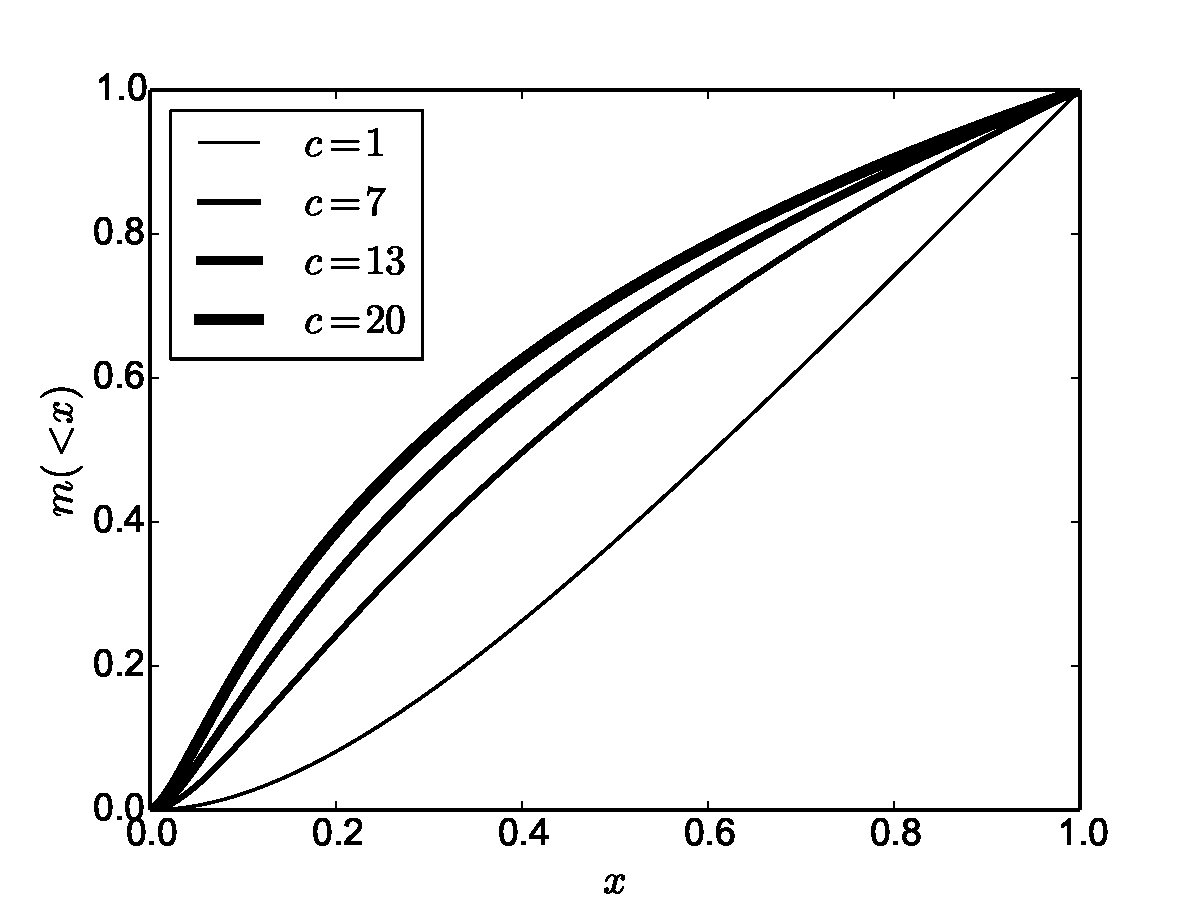
\includegraphics[width=0.48\textwidth]{nfw_normalized.pdf}
\end{center}
\caption{Mass profiles of several haloes with different concentrations
    \label{fig:profiles}}
\end{figure}


\section{A Bayesian Approach to Halo Fitting}
\label{sec:method}


We proceed to find the value of the concentration parameter that
best describes the simulation data, following the model in
Eq. (\ref{eq:profile}). We use the integrated mass profile because it
allows us to use the data directly with the simulation without binning
the particle positions and estimating a density.

We construct the integrated mass profile by ranking the particles by
their increasing distance to the center of the halo. Once they are ranked,
the total mass at a radius $r_i$, increases by $m_p$, where $r_i$ is
the position of the $i$-th particle and $m_p$ is the mass of the
computational particle.  We define the center of the halo to be  at
the position of the particle with the lowest gravitational
potential. In the process of building the mass profile we discard the
particle at the center.

We stop the construction of the integrated mass profile once we arrive
at an average density of $\Delta_h\bar{\rho}$. This radius marks the
virial radius and the virial mass. We divide the total mass enclosed
mass $M_i$ and the radii $r_i$ by these values to obtaine the
dimensionless variables $x_i$ and $m_i$. 

Using these positions and masses we define the following $\chi^2$ function

\begin{equation}
\chi^2(c) = \sum_{i}[\log m_i - \log m(< x_i;c)]^2, 
\end{equation}
%
where $m(<x_i;c)$ corresponds to the values in Eq.(\ref{eq:profile}) at
$x=x_i$ and a given value of the concentration parameter $c$.

Finally we use a Metropolis-Hastings algorithm to sample the likelihood
function distribution defined by ${\cal L}(c)=\exp(-\chi^2(c)/2)$ to
find the optimum value of $c$ and its associated uncertainty
$\sigma_c$. 

\section{Numerical Experiments}

\subsection{Mock Halos}

We generate $100$ mock halos with concentration values randomly
placed in the range $1<c<10$. Each one of the halos is generated with
four different total particle numbers: $20$, $200$, $2000$ and $20000$.

The method we use to generate the halos is based on the integrated
mass profile. Given the number of particles $n$ and the concentration
$c$ we define the mass element as $\delta m = 1/n$ (this corresponds
to the mass of each particle such that the total mass is one). Then
for each number $k$ from $1$ to $n$ we find the value of $r$ such that
the difference 
%
\begin{equation}
m(<r;c)-k \cdot \delta m 
\end{equation}
%
is zero using Ridders' method. This value of $r$ is the radius of
the $k$th particle of the generated halo, then polar and azimuthal
angles $\theta$ and $\phi$ are randomly generated. Finally these three
coordinates are transformed into cartesian coordinates
$(r,\theta,\phi) \rightarrow (x,y,z)$. This process is repeated $n$
times in order to generate the $x,y,z$ coordinates for each particle. 

\subsection{Simulation Data}
\label{sec:data}

We use data from the MultiDark cosmological volume. This simulation
follows the non-linear evolution of a dark matter density field
sampled with $2048^3$ particles over a cubic box of $1000$ \hMpc on a
side. The data is publicly available, more details about the structure
of the database and the simulations can be found in
\citep{2013AN....334..691R}. 

We select a sample of halos in a cubic sub-volumne of $100$ \hMpc on a
side centered on the most massive halo in the simulation at
$z=0$\footnote{This corresponds to the \texttt{miniMDR1} database in
  the MultiDark webpage}. We select first all the halos at $z=0$
detected with a Friends-of-Friends (FoF) algorithm with masses in the
interval $10^{11}\leq M_{\rm FoF}/\hMsun \leq 10^{15}$. The FoF
algorithm ran with a linking length of $0.17$ times the average
interparticle distance. This choice translates into an overdensity
$\Delta_h\sim 400-700$ that is dependent on the halo concentration
\citep{More2011}.

For each selected halo with the previous procedure we select from the database
all the particles that belong to it. From the particles we follow the
procedure spelled out in Section \ref{sec:method} with $\Delta_h=740$
(corresponding to $200$ times the critical density) to find the
halo concentration. Finally, we store the values obtained for the
virial radius, virial mass and concentration. 


\section{Results}
\label{sec:results}


\subsection{Mock Halos}
\label{sec:results_mocks}

\begin{figure}
\begin{center}
  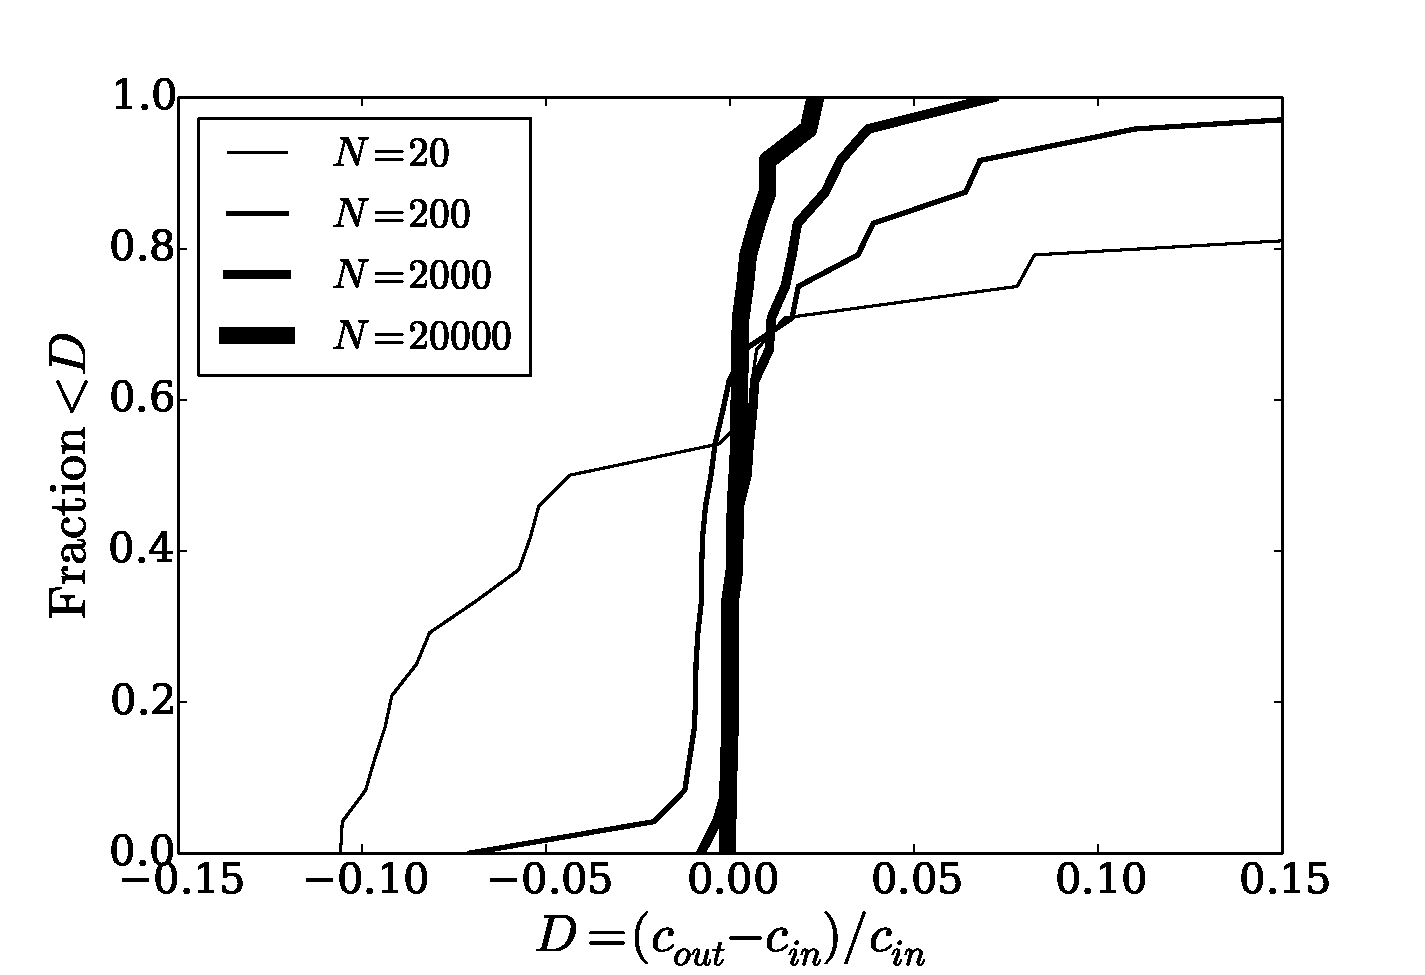
\includegraphics[width=0.48\textwidth]{percentual_diff.pdf}
\end{center}
\caption{Cumulative distribution of the fractional difference between
  the input concentration in the mock halo generator, $c_{in}$ and the
  measurement by our MCMC code, $c_{out}$. Each curve corresponds to
  halos generated with a different number of particles, $N$.
    \label{fig:results_mocks}}
\end{figure}


In Figure \ref{fig:results_mocks} we show the integrated distribution
percentual difference between the concentration measured with our
fitting method $c_{out}$ in comparison with the concentration used to
generate the mock halos, $c_{in}$, $D=(c_{in}-c_{out})/c_{in}$. Then we can see that as the number of particles increases, the curve becomes more pronounced at 0. Showing that for most of the halos $c_{in}$ is very similar to $c_{out}$.


\subsection{Simulation Data}
\label{sec:results_mocks}

\section{Discussion}
\label{sec:discussion}

\subsection{Comparison against other methods}
We compared this method against two methods: The first one consists in using shells for estimating the density in function of the radius and using the same MCMC method for fitting and the second one consists in using the circular velocity $V(r)=\sqrt{GM(<r)/r}$ and the relation for the NFW profile
\begin{equation}
\frac{V_{max}}{V(r_{v})} = \sqrt{\frac{0.216c}{M(r_{v};c)}}
\end{equation}
Where $V_{max}$ is the maximum velocity, to find the value of the concentration.

\begin{figure}
\begin{center}
  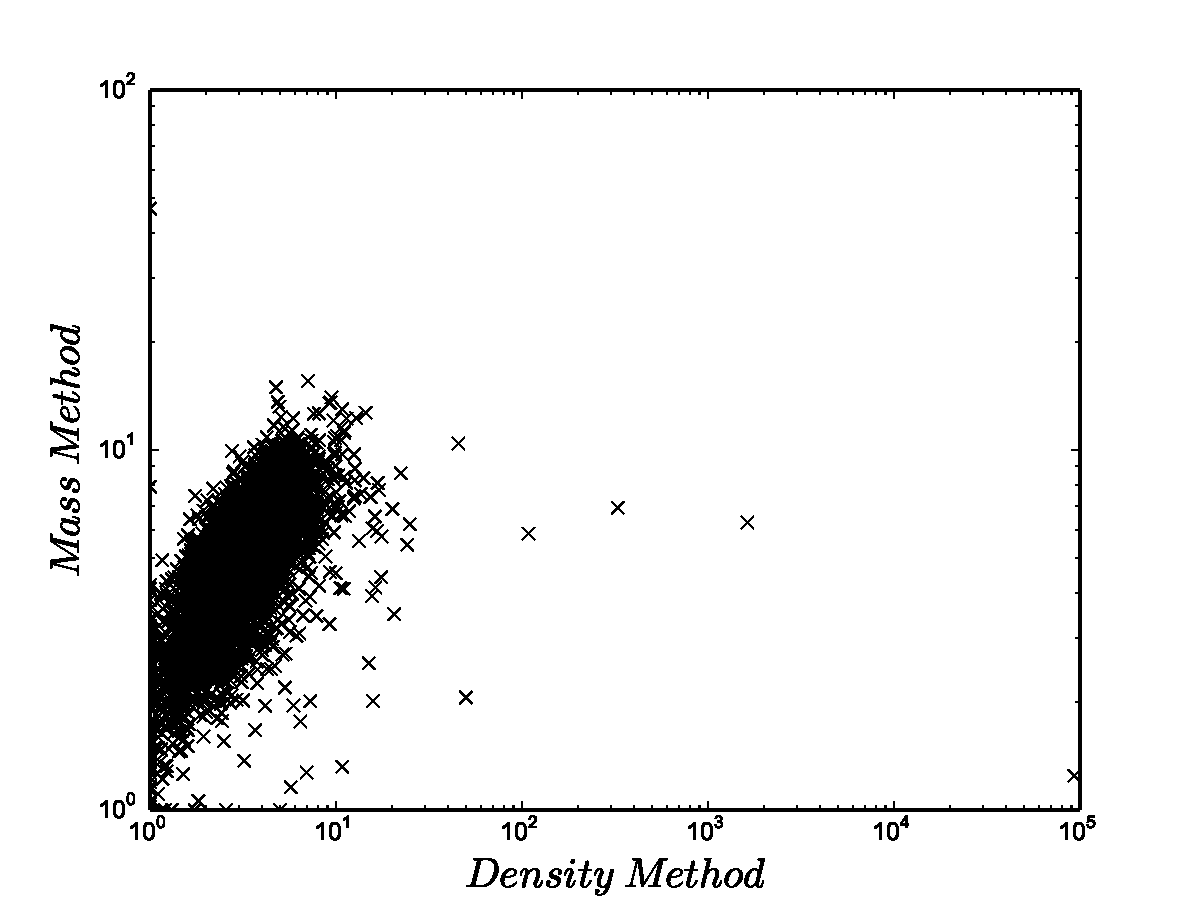
\includegraphics[width=0.48\textwidth]{density-mass.pdf}
\end{center}
\caption{Concentration obtained from the mass method against the one obtained in the density method
    \label{fig:density-mass}}
\end{figure}
\begin{figure}
\begin{center}
  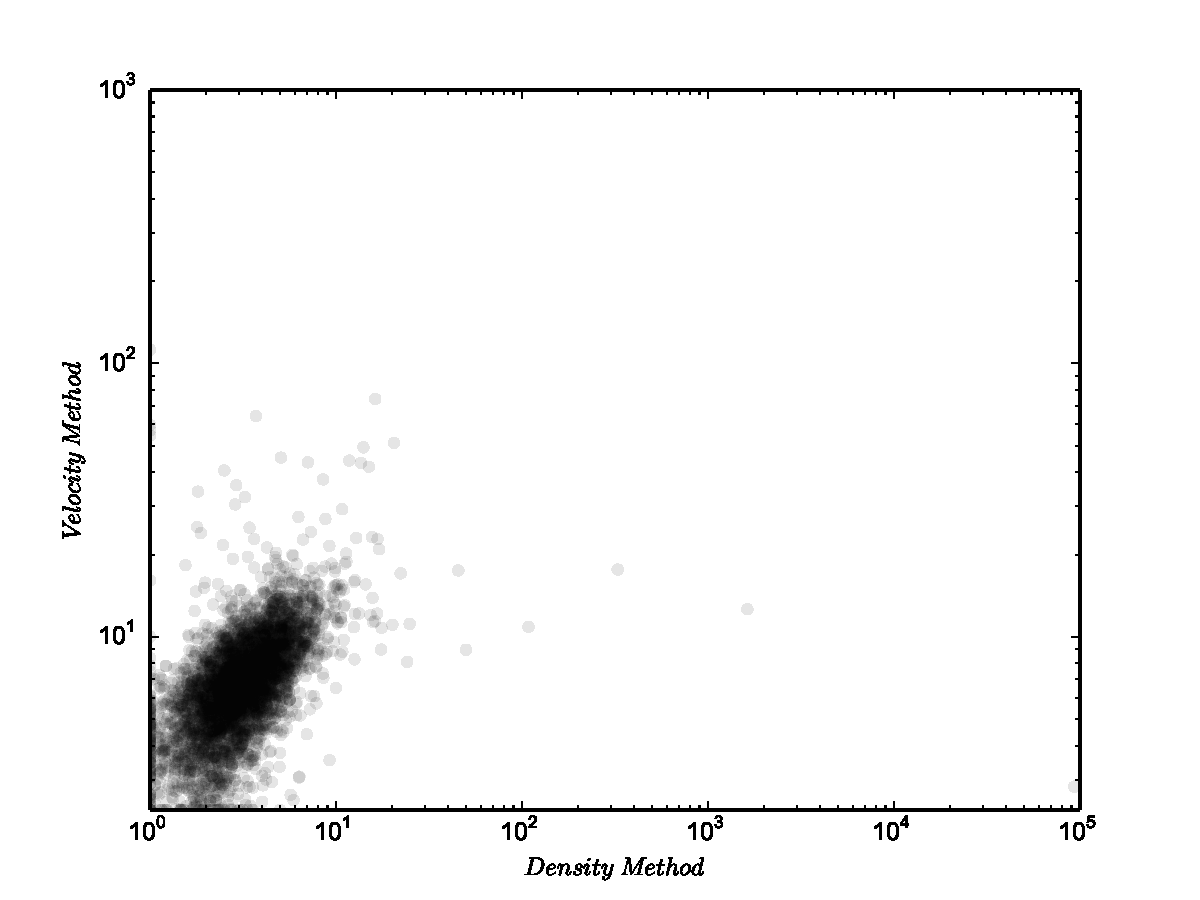
\includegraphics[width=0.48\textwidth]{density-velocity.pdf}
\end{center}
\caption{Concentration obtained from the velocity method against the one obtained in the density method
    \label{fig:density-velocity}}
\end{figure}
\begin{figure}
\begin{center}
  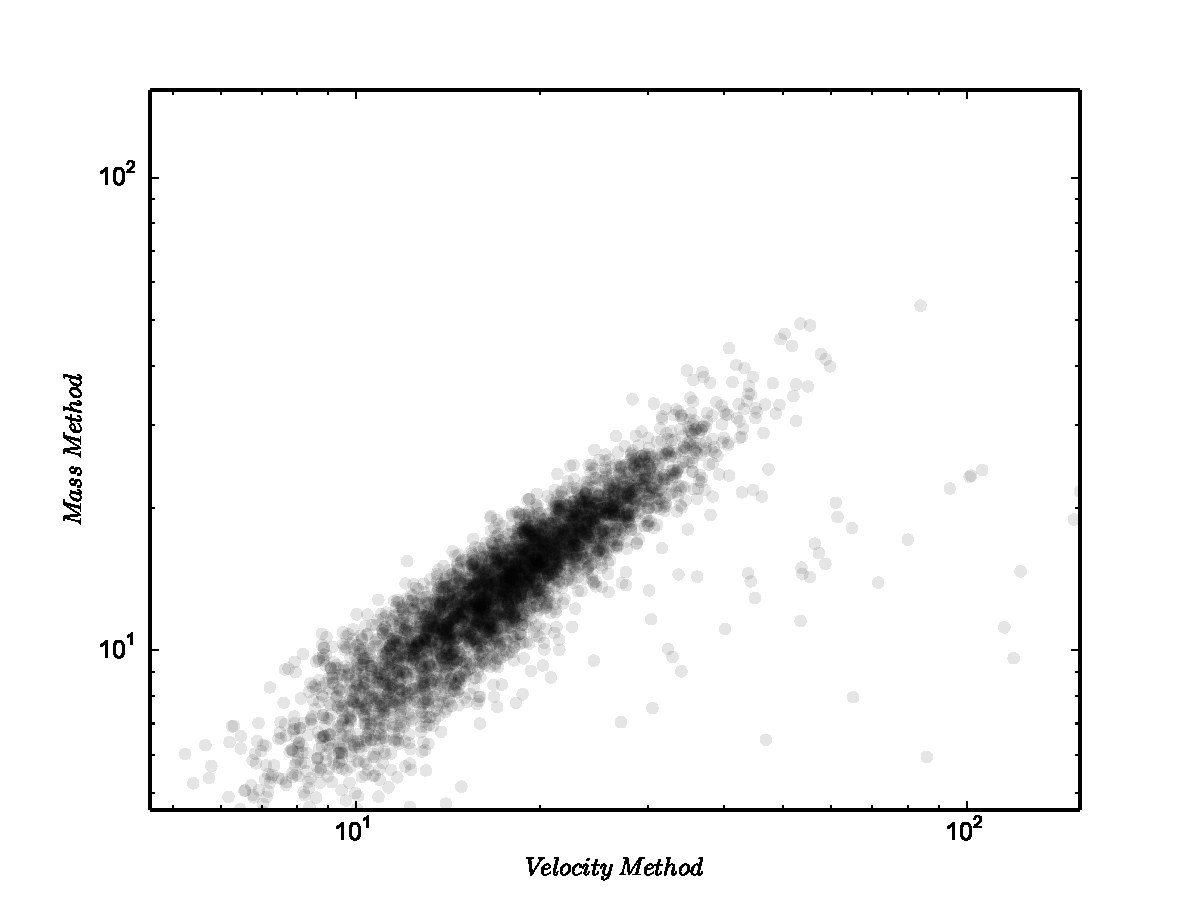
\includegraphics[width=0.48\textwidth]{velocity-mass.pdf}
\end{center}
\caption{Concentration obtained from the mass method against the one obtained in the velocity method
    \label{fig:velocity-mass}}
\end{figure}

We tested the three methods using the same data from the Mock Halos test. In order to see the accuracy of each method depending on the number of particles we define 

\begin{equation}
\xi=\frac{1}{N}\sum\left|\frac{c_{org}-c_{obt}}{c_{org}}\right|
\end{equation}

Where $c_{org}$ and $c_{obt}$ are the original and obtained concentrations respectively and $N$ the number of haloes with a certain number of particles. Then we calculate $\xi$ for each number of particles (20, 200, 2000 and 20000).

\begin{figure}
\begin{center}
  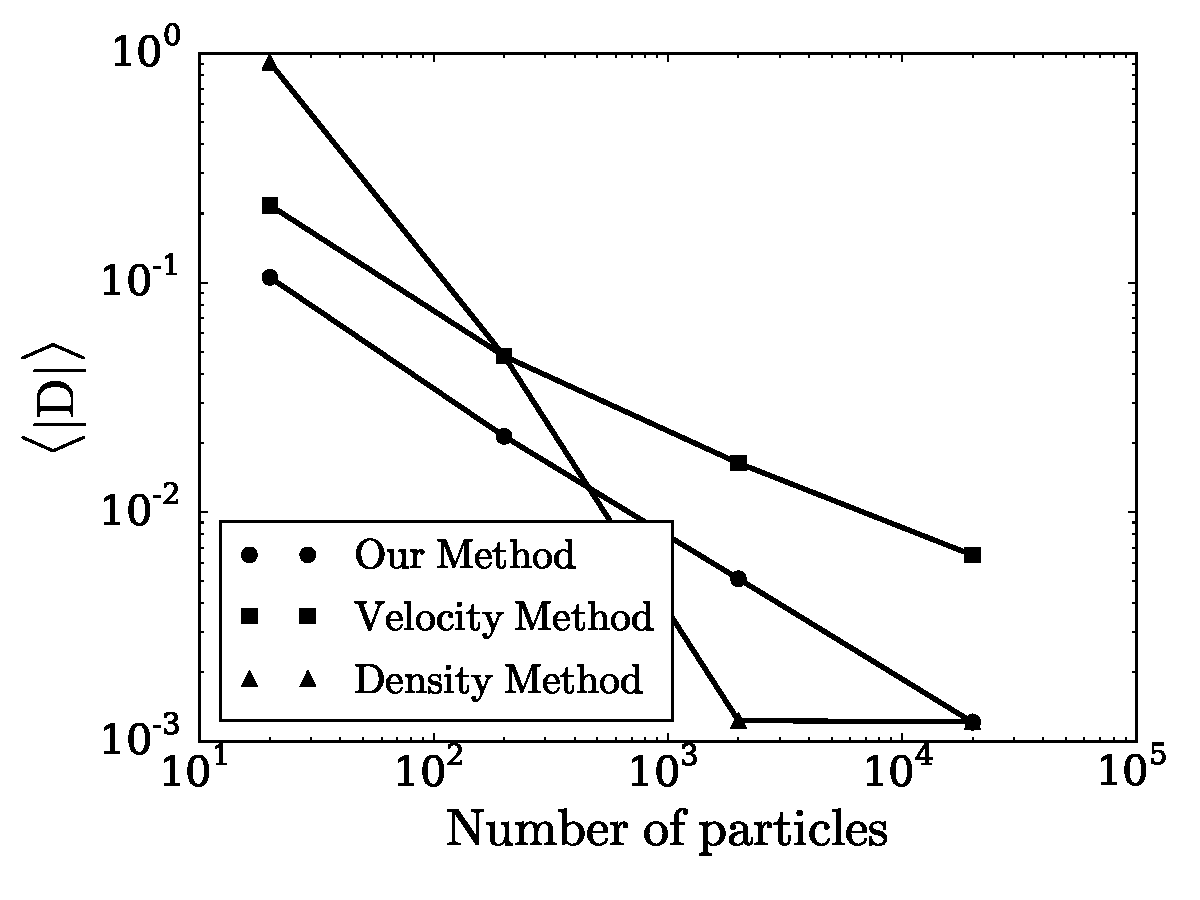
\includegraphics[width=0.48\textwidth]{error.pdf}
\end{center}
\caption{Relative error Against number of Particles
    \label{fig:error}}
\end{figure}

In Figure \ref{fig:error} we plotted $\xi$ for the three methods. We consider that $\xi$ is a good estimate because it is standardized, giving equal weight to all errors regardless of the magnitude of the concentrations or the number of halos. On the other hand we have that $\xi$ decreases quite fast with the number of particles and is more precise in any case that the other methods.

\subsection{Concentration as a function of halo mass}
Aditionally we compared those three methods plotting the concentration as a function of the number of particles of each halo 

\begin{figure}
\begin{center}
  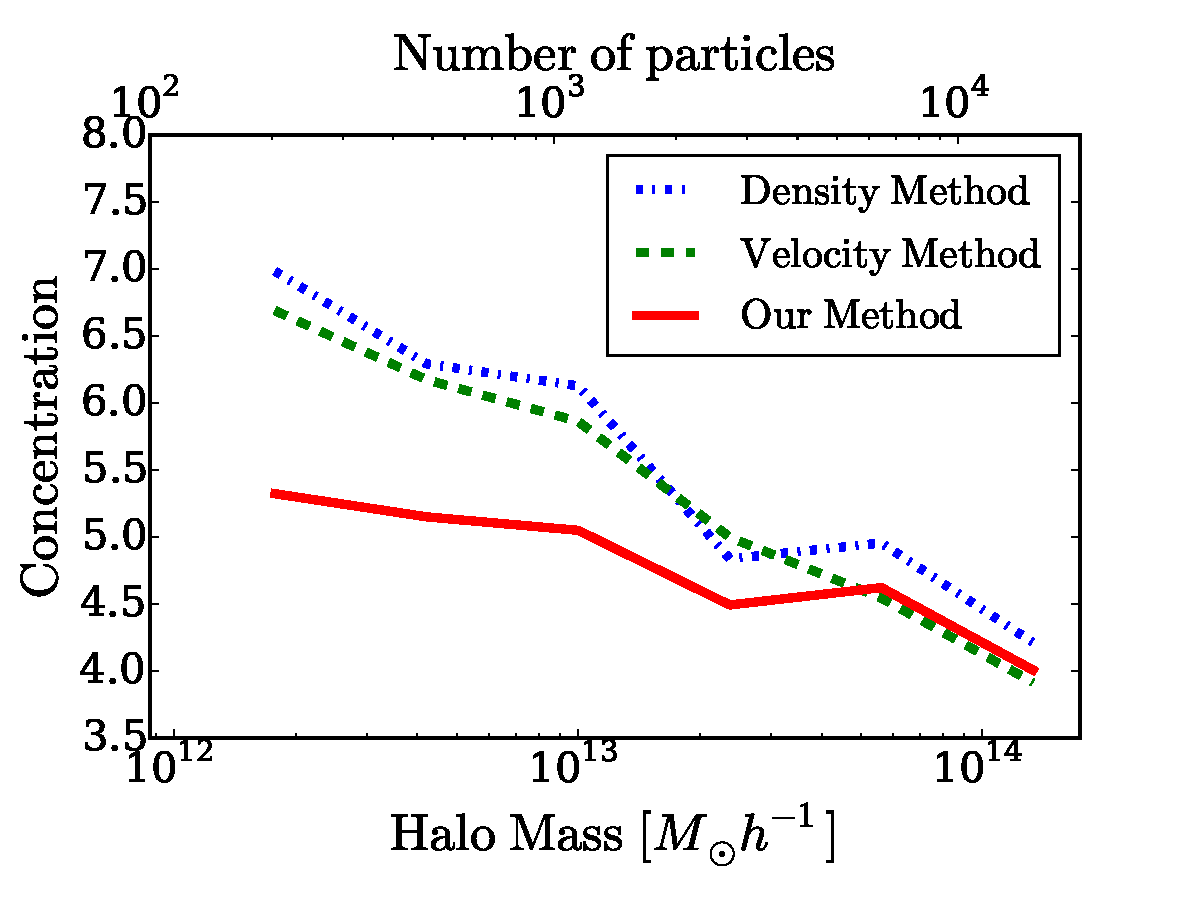
\includegraphics[width=0.48\textwidth]{concentration.pdf}
\end{center}
\caption{Concentration against number of particles
    \label{fig:concentrations}}
\end{figure}

The bold lines in Figure \ref{fig:concentrations} corresponds to the median and the thinner lines corresponds to the quartiles.
\subsection{Implication for comparisons against observations}
FIXME: Ask to Jaime


\section{Conclusions}
\label{sec:conclusions}
FIXME: Ask to Jaime

\bibliographystyle{mn2e}
\bibliography{references}

\end{document}
